\chapter{Introducción}

El objetivo de este proyecto es construir un software con el que poder visualizar e interactuar con los datos DICOM obtenidos al someter a una escultura a una Tomografía Computarizada (TAC o TC). 

Para ello se hará uso de VTK, que proporciona una serie de librerías en C++ para facilitar operaciones sobre datos DICOM, y de Qt, para la Interfaz Gráfica de Usuario (GUI).

Antes de empezar con el proyecto en sí, se definirán conceptos como DICOM o TC que se usarán a lo largo de éste y conviene saber lo que son. 

También se comentará brevemente qué materiales se utilizan en las esculturas de madera policromadas así como su proceso de elaboración y los posibles factores de deterioro que pueden presentar.

\section{Obtención de datos DICOM mediante una TC}

DICOM (\textit{Digital Imaging and Comunication in Medicine}) es el estándar internacional para manejar, visualizar, almacenar, imprimir y transmitir imágenes de pruebas médicas (ISO12052) \cite{about_dicom}. 

Al contrario de lo que se puede pensar en un principio, DICOM es más que un formato de imagen, es un protocolo que abarca la transferencia, el almacenamiento y la visualización \cite{dicom_intro_and_guide}.

Pese a que su uso está mayoritariamente extendido en el campo en el que nació (la medicina) para obtener imágenes de cortes de partes del cuerpo de un paciente con fines diagnósticos, se puede usar en otros, como el de la restauración de bienes culturales, como es el caso de este proyecto.

En un archivo DICOM hay almacenado, además de metadatos, una imagen \cite{dicom_classes_vtk} (Figura \ref{fig:prostate_dicom}).

\begin{figure}[H]
	\centering
	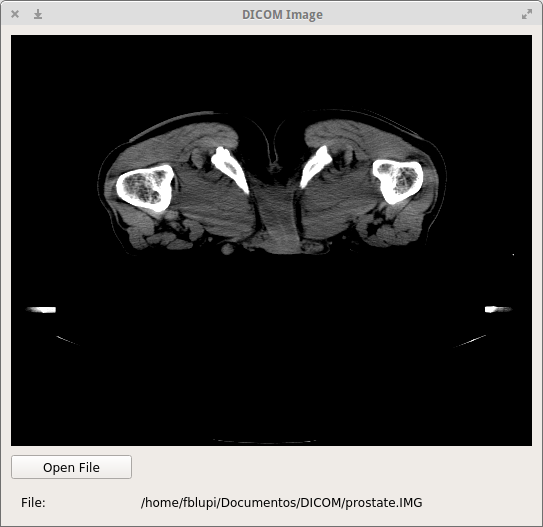
\includegraphics[width=10cm]{imagenes/prostate_dicom}
	\caption{Imagen DICOM de una próstata visualizada con un programa diseñado para visualizar archivos DICOM}
	\label{fig:prostate_dicom}
\end{figure}

Cuando se realiza una TC se obtienen una serie de imágenes 2D (Figura \ref{fig:brain_dicom_serie}) de cortes del objeto al que se le realiza el escáner. Éstas imágenes se encapsulan en archivos DICOM, y con todas ellas se puede pasar a un espacio en 3D y llegar a construir un modelo volumétrico en el que para cada voxel (Volumetric Pixel) se tiene el valor de densidad del objeto en ese punto.

El cómo se obtienen las imágenes con una TC no es objeto de estudio de este proyecto, por lo que no se entrará en mucho detalle. En muy resumidas cuentas, el aparato emite un haz de rayos X desde distintos ángulos al objeto y unos sensores recogen la radiación que absorbe en cada una de estas emisiones. Obteniendo el resultado final del promedio de todas las mediciones que realizan los sensores \cite{tac}. 

\begin{figure}[H]
	\centering
	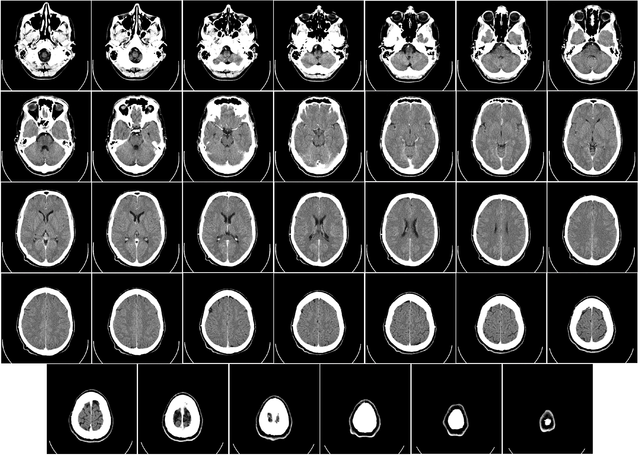
\includegraphics[width=10cm]{imagenes/brain_dicom_serie}
	\caption{Serie de imágenes DICOM extraídas de una TC realizada a un cerebro}
	\label{fig:brain_dicom_serie}
\end{figure}

Para renderizar la imagen con una técnica de Direct Volume Rendering (DVR) hay que darle a cada voxel un valor de color y opacidad. Esto se realizará con lo que se denomina función de transferencia (de la que se hablará exhaustivamente más adelante) que a partir de los valores de densidad y gradiente de cada voxel obtiene un valor de color y opacidad y mediante \textit{ray casting} o cualquier otra técnica de DVR se consigue el color para un pixel. Aquí es donde entrará en juego VTK, una librería que ayudará enormemente en la realización de estas tareas.

\section{VTK} 

VTK es una librería gráfica orientada a objetos de alto nivel desarrollada por la compañía Kitware. Permite su uso en lenguajes compilados como C++ y Java o interpretados como Tcl y Python. Debido a los años que lleva desarrollándose, desde 1993 hasta la actualidad, se ha convertido en una librería enorme y compleja, pero al mismo tiempo potente \cite{intro_medical_vtk_bioimage}. Esto hace que su curva de aprendizaje tenga un inicio lento. Pero merece la pena su uso porque aunque cueste aprender, el tiempo invertido es mucho menor que al que habría que invertir para realizar las operaciones tan complejas que facilita.

\section{Esculturas de madera policromadas}

\subsection{Historia}

El tallado es el método de elaboración de esculturas más antiguo conocido. Se ha tallado en distintos materiales (madera, piedra, marfil...). Pero la madera, por condiciones como su ligereza o la facilidad de ensamblado entre distintas piezas, ha sido uno de los materiales más utilizados.

Se conoce que desde el Antiguo Egipto ya se realizaban esculturas de madera pero es a partir del siglo XI cuando comienza su proliferación. Y desde este momento comienzan a producirse mejoras en las técnicas y herramientas utilizadas durante el proceso del tallado \cite{tc_esculturas}.

\subsection{Maderas más utilizadas}

Dependiendo del tipo de escultura se utilizan maderas blandas o duras. Si la escultura es más pequeña y contiene más detalles se utilizará un tipo de madera más dura.

No obstante, en la elección también tiene mucha influencia la situación geográfica al utilizarse maderas autóctonas \cite{tc_esculturas}:

\begin{itemize}
	\item \textbf{Italia}: Álamo y chopo.
	\item \textbf{Francia}: Nogal y castaño.
	\item \textbf{Países Bajos}: Roble y encina.
	\item \textbf{España}: Pino de Flandes, cedro de la Habana, castaño, tejo, álamo, nogal, ciprés, boj, pino silvestre y algunos frutales como el peral.
\end{itemize}

Además de la madera, una escultura de madera policromada, puede contener varios materiales como el estuco o el metal de los clavos utilizados.

\subsection{Defectos de la madera}

Entre los defectos de la madera se pueden encontrar \cite{tc_esculturas}:

\subsubsection{Grietas o fendas}
Según la UNE-EN 844-9 se denomina grieta o fenda a ``toda separación de las fibras (raja o hendidura) en dirección longitudinal". Según su origen, pueden ser de distintos tipos: 

\begin{itemize}
	\item \textbf{Acebolladuras o \textit{colainas}}: Hay una discontinuidad entre los anillos de crecimiento.
	\item \textbf{Superficiales o de desecación}: Producidas por el calor, provocan un deterioro en las zonas externas del tronco del árbol dejando la madera desprotegida. Provocan grietas en sentido longitudinal.
	\item \textbf{De heladura}: Producidas por una helada dañan la superficie e interior del tronco. Provocan grietas radiales.
	\item \textbf{De viento}: Originadas por la acción de un fuerte viento. Provocan grietas longitudinales y transversales.
\end{itemize}

Además de estos procesos naturales, se pueden producir grietas durante procesos como el secado que provocan una separación de las fibras.

\subsubsection{Fibras reviradas y entrelazadas}

Las fibras se encuentran normalmente orientadas en paralelo al eje principal del tronco, pero en ocasiones pueden presentar nudos que alteran la dirección de éstas.

\subsubsection{Nudos}

La UNE 56.521 define nudo como ``anomalía local de la estructura de la madera producida por la parte inferior de una rama que va quedando englobada en el tronco a medida que se producen los crecimientos de este". Existen distintos tipos:

\begin{itemize}
	\item \textbf{Adherente, vivo, fijo o sano}: Definido por la UNE 56.521 como ``aquel cuyos tejidos son solidarios con los de la madera que los rodea debido a ser formado por una rama viva".
	\item \textbf{Suelto, saltadizo, muerto o seco}: Definido por la UNE 56.521 como ``aquel en que los tejidos de la rama que lo producen no son solidarios con los de la madera que los rodea y suelen separarse".
\end{itemize}

\subsubsection{Núcleos de resina}

Son cavidades entre los anillos de crecimiento producidos frecuentemente por nudos.

\subsubsection{Factores de deterioro de tipo biótico}

Además de las alteraciones que ya presenta la madera, existen otros factores que también influyen como la humedad y la temperatura o el ataque de insectos xilófagos y hongos.

Los insectos xilófagos se nutren de madera seca y favorecen a su desarrollo una humedad relativa y temperaturas no muy bajas. Estos producen daños rompiendo las fibras de la madera.

Los hongos son microorganismos que pueden desarrollarse en la superficie o en el interior de la madera, haciendo que pierda humedad, reduciendo su tamaño y deformándose. Existen tres tipos distintos de degradación tras un ataque de hongos: pudrición blanca, parda o seca y blanda.

\subsection{Proceso de tallado}

El proceso de tallado se podría definir como una técnica sustractiva en la que a partir de una pieza se obtiene una forma concreta.

Un método puede ser utilizar un único bloque de madera. En ocasiones ahuecado por el reverso para contrarrestar fuerza y movimiento de la madera, y, en cierto modo, aligerando el peso.

A partir del siglo XVI empieza a utilizarse con más frecuencia otro método en el que a partir de un bloque principal se ensamblan diferentes piezas generando un bloque más grande, denominado embón, con la forma y el tamaño de la imagen a esculpir. A partir de éste se comienza el tallado.

A partir del Barroco se mejora esta técnica realizando ensamblados en hueco para evitar el posterior ahuecado \cite{tc_esculturas}.

\section{Trabajos previos}

Como ya se ha comentado anteriormente, el uso de las imágenes obtenidas con las TCs está muy extendido en el campo de la medicina, aunque puede ser usado en otros. 

Ha tenido bastante repercusión en estudios anatómicos del estado actual de momias \cite{mummies} y para realizar reconstrucciones de su posible estado anterior \cite{mummies_reconstruction}.

En el caso de estudio de este proyecto, la restauración de bienes culturales, obviamente, también puede aplicarse.

Tradicionalmente, se han utilizado radiografías para examinar el estado de las esculturas, pero tienen sus limitaciones como la superposición de planos. El uso de TCs como técnica de estudio no destructiva hace que se puedan obtener resultados que permitan realizar exámenes más precisos y exhaustivos a los restauradores sin dañar la escultura \cite{tc_esculturas}.

Se podría hacer uso de herramientas médicas como OsiriX \cite{osirix}, AMILab \cite{amilab} o RadiAnt; pero proporcionan \textit{presets} para visualizar materiales de los que están compuestos el organismo humano y la mayoría de ellas tienen un precio de licencia bastante elevado.

También se podrían utilizar herramientas más genéricas como 3DSlicer \cite{slicer}, desarrollada por la misma compañía que VTK. No obstante, tiene muchas funcionalidades que no utilizarían los restauradores y hacen de ella una herramienta demasiado compleja.

Incluso podrían hacer uso de software específico para la visualización de esculturas, aunque hay muy pocas herramientas que tengan funcionalidad para trabajar con conjuntos de datos volumétricos. La más referenciada es Hyper3D \cite{hyper3d} pero los resultados obtenidos no son buenos (Figura \ref{fig:hyper3d_results}).

\begin{figure}[H]
	\centering
	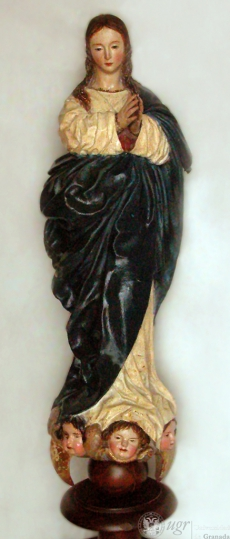
\includegraphics[height=9cm]{imagenes/inmaculada_concepcion_real}
	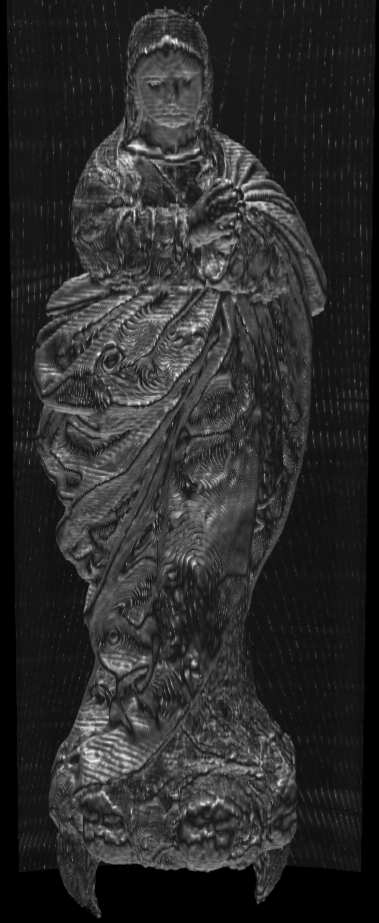
\includegraphics[height=9cm]{imagenes/inmaculada_concepcion_hyper3d}
	\caption{A la izquierda escultura de la Inmaculada Concepción. A la derecha su reconstrucción volumétrica usando Hyper3D y su \textit{preset} para madera}
	\label{fig:hyper3d_results}
\end{figure}

\section{Motivación}

El resultado insatisfactorio obtenido con las herramientas disponibles ha motivado la idea de desarrollar \myTitle, un software creado para que los restauradores puedan examinar esculturas de madera policromadas y así conocer los materiales de los que están compuestas, su estructura interna, detectar si ha sufrido un ataque de tipo biótico o si presenta cualquier otro daño.

Conocer la estructura interna de la escultura que se somete a examen es de gran ayuda para realizar tareas de conservación y restauración de más calidad sobre esta \cite{tc_esculturas}.

El software incluirá una serie de \textit{presets} para poder visualizar unos u otros materiales sin que el usuario tenga por qué conocer los valores de densidad de estos para crear una función de transferencia que los visualice, pero proporcionando también un editor de funciones de transferencias con el que los usuarios más avezados puedan crear sus propios \textit{presets} y exportarlos para que puedan ser utilizados por los demás.
